%===============================================================================
% $Id: ifacconf.tex 19 2011-10-27 09:32:13Z jpuente $
% Template for IFAC meeting papers
% Copyright (c) 2007-2008 International Federation of Automatic Control
%===============================================================================
\documentclass{ifacconf}

\usepackage{graphicx}      % include this line if your document contains figures
\usepackage{natbib}        % required for bibliography
\usepackage{subfigure}
\usepackage{enumerate} 
%===============================================================================
\begin{document}
\begin{frontmatter}

\title{THE EMBEDDED ELECTRONICS SYSTEM OF DORIS: A MOBILE ROBOT FOR INSPECTION AND MONITORING OF
OFFSHORE FACILITIES\thanksref{footnoteinfo}}
% Title, preferably not more than 10 words.

\thanks[footnoteinfo]{This work is supported primarily by Petrobras S.A. and
Statoil Brazil Oil \& Gas Ltda under contract COPPETEC 0050.0079406.12.9
(ANP-Brazil R \& D Program), and in part by the Brazilian research agencies CNPq
and FAPERJ}

\author[1]{Renan S. Freitas}
\author[1]{Marco F. S. Xaud}
\author[1]{Ighor Marcovistz}
\author[1]{Alex Neves}
\author[1]{Guilherme P. S. Carvalho}
\author[1]{Liu Hsu}
\author[1]{Eduardo V. L. Nunes}
\author[1]{Fernando C. Lizarralde}
\author[1]{Gustavo Freitas}
\author[1]{Eduardo A. B. da Silva}
\author[2]{Maurício Galassi}
\author[3]{Anders R{\o}yr{\o}y}
\author[1]{Ramon R. Costa}

%\address[First]{Federal University of Rio de Janeiro, COPPE, Rio de
%Janeiro, Brazil}
%\address[Second]{Federal University of Rio de Janeiro, COPPE, Rio de
%Janeiro, Brazil}
%\address[Third]{Federal University of Rio de Janeiro, COPPE, Rio de
%Janeiro, Brazil, (e-mail: )}
%\address[Forth]{Federal University of Rio de Janeiro, COPPE, Rio de
%Janeiro, Brazil}
%\address[Fifth]{Electrical
%Engineering Department, COPPE UFRJ, Rio de Janeiro, Brazil, (e-mail: )}
%\address[Sixth]{Electrical
%Engineering Department, COPPE UFRJ, Rio de Janeiro, Brazil, (e-mail: )}
%\address[Seventh]{Electrical
%Engineering Department, COPPE UFRJ, Rio de Janeiro, Brazil, (e-mail: )}
%\address[Eigth]{TPD RD New Development Solutions, Statoil ASA}
%\address[Nineth]{Research and Development Center, Petrobras/CENPES, Rio de
%Janeiro, Brazil}
%%\address[Tenth]{Mathematical Sciences and Technology Department, Norwegian
%University of Life Sciences, Oslo, Norwegian }
%%\address[Eleventh]{Electrical
%Engineering Department, COPPE UFRJ, Rio de Janeiro, Brazil, (e-mail: )}
 \address[1]{Electrical
 Engineering Department, COPPE UFRJ, Rio de Janeiro, Brazil}
 \address[2]{Research and Development Center, Petrobras/CENPES,
 Rio de Janeiro, Brazil}
 \address[3]{TPD RD New Development Solutions, Statoil ASA}
% % \address[]{Mathematical Sciences and Technology Department, Norwegian
% % University of Life Sciences, Oslo, Norwegian }



\begin{abstract}                % Abstract of not more than 250 words.
DORIS is a research project which endeavors to design and implement a mobile
robot for remote supervision, diagnosis, and data acquisition on offshore
facilities. The proposed system is composed of a railguided robot capable of
carrying different sensors through the inspected area. This paper presents a
general overview of the robot, a description of the developed embedded
electronics, power supply system and software architecture. Initial results
with teleoperated navigation validate the concepts considered so far and
rise several challenges for future works.
\end{abstract}

\begin{keyword}
mobile robots; field robotics..
\end{keyword}

\end{frontmatter}
%===============================================================================

\section{Introduction}
The Oil \& Gas demand will grow rapidly in the next decades (\cite{wna}) and the
need to obtain the resources from hostile environments will increase the
operation cost and rise the employee salary. In order to be competitive
and to improve their profit, oil \& gas companies are looking for new
technologies to reduce the labor cost. Using robotics in inspection, maintenance
and repair could greatly improve safety and efficiency. 

In the specific case of Brazil, the Oil \& Gas industry is growing at high pace.
The recent discoveries of big oil fields in the pre-salt layer off the Brazilian
coast, located 300 km from the shore at depths of 5000 to 7000 km, motivates the
development of an offshore  production system with a high degree of automation
based on advanced robotics systems (\cite{OTC}).

The work conditions on offshore installations such as unfriendly atmosphere,
unsheltered environment, heavy wheather, extreme temperatures, constraint space,
and the logistical issues are serious financial obstacles for oil \& gas
companies. It is highly expensive to have people working on the rig as they must
be housed and protected, there are costs with personal benefits like health
care, and the companies must have the possibility to evacuate personnel quickly,
in the case of emergency.

Recent studies forecast a substantial decrease in the level of human operation
and an increase in automation on future offshore oil fields
(\cite{skourup2009robotized}).The studies also point out the potential increase
in efficiency and productivity with robot operators, besides the improvement of
Health, Safety, and Environment (HSE) conditions, as robots can replace humans
in tasks performed in unhealthy, hazardous, and confined areas ~\cite{pal}.

\cite{chen} investigates the challenges of robotics and automation in oil
\& gas industry. The most important requirements for robotic systems are:
\begin{itemize}
\item The atmospheric conditions on offshore platforms are quite unfriendly. The
hydrocarbon resources can generate explosive, toxic and corrosive gases. The
robot should be explosion-proof.
\item Corrosive environments: splashy salty water, saltyair and corrosive
chemicals.
\item Heavy weather: wind with high speed, squalls, rain and hail. The
significant variations on ambient temperature and relative humidity up to
100\%. Possibly highly radiant heat from process equipment and direct sunlight. 
\item Constraint space and/or walkways. Complex structures such as pipes,
flanges, tanks, stairways and many more.
\end{itemize}

There are different kinds of robots in the oil \& gas industry. Underwater
pipeline repair robotic systems; robots for inpection of valve and lever
position; gas level or leakage and acoustic anomalies monitoring; robots for
identify and locate fire; 

The Fraunhofer inspection robot (MIMROex, \cite{mimroex}) was developed and
tested by the Fraunhofer Institute of Manufacturing Engineering and Automation (IPA). The
robot is capable of safe navigation in offshore environments, and it
autonomously executes the inspection tasks.

The Carnegie Mellon University inspection robot, Sensabot (\cite{sensabot}), was
designed for severe weather and unfriendly atmosphere with corrosive, toxic and explosive
gasses. The robot includes the following sensors: (i) hydro carbon sensor; (ii)
pan/tilt/zoom camera for remote operations; (iii) temperature sensors; (iv)
vibration sensor for pumps, motors and bearings inspection; (v) microphone to
detect audible machinery problems; (vi) video camera to detect obstacles.

The SINTEF Topside Robotic System, developed in the robotic lab facility in
Trondheim, is an intelligent instrumentation system to enable onshore operators
to monitor and control all of the platform's processes
(\cite{kyrkjebo2009robotic}).




% 
% Safety and efficient operation are imperative factors to offshore production
% sites and a main concern to all Oil \& Gas companies. A promising solution to
% improve both safety and efficiency is to increase the level of automation on
% the platforms by introducing robotic systems.
% 
% During the last decade, several Oil \& Gas companies, research groups, and
% academic communities have shown an increasing interest in the use of robots for
% operation on offshore facilities.
% 
% Recent studies forecast a substantial decrease in the level of human operation
% and an increase in automation on future offshore oil fields
% ~\cite{skourup2009robotized}.The studies also point out the potential increase
% in efficiency and productivity with robot operators, besides the improvement of
% Health, Safety, and Environment (HSE) conditions, as robots can replace humans
% in tasks performed in unhealthy, hazardous, and confined areas ~\cite{pal}.
% In~\cite{abb}, it is considered the use of robots in Oil \& Gas offshore
% facilities in operations that require both high precision and strength,
% regardless of weather conditions.
% 
% In the specific case of Brazil, the Oil \& Gas industry is growing at a high
% pace, mainly due to the recent discoveries of big oil fields in the pre-salt
% layer off the Brazilian coast. These oil reservoirs are located farther than
% 300 km from the shore at depths of 5000 to 7000 km. These factors,
% especially the large distances, motivate the development of an offshore
% production system with a high degree of automation based on advanced robotics
% systems.

% Among the research groups interested in offshore robotics, \emph{Fraunhofer
% IPA} is pioneer in proposing and demonstrating the applicability of mobile
% robots for offshore inspection and maintenance tasks \emph{in
% loco} ~\cite{mimroex2}. One example is MIMROex ~\cite{mimroex}, capable of
% navigating safely, building maps, and executing inspection tasks autonomously
% throughout the topside of platforms.
% 
% Another robotic device applied in offshore environments is Sensabot
% ~\cite{sensabot}, capable of safely inspect and monitor hazardous and remote
% production facilities. The robot can sustain high temperatures, is able to
% reach areas with difficult access, and is certified to operate in explosive and
% toxic environments.

% SINTEF-ICT is another group interested in manipulators applied to the oil and
% gas industry. Inspection and maintenance operations in a simulated production
% process are performed by the cooperation of a gantry-mounted manipulator and a
% floor-mounted robot ~\cite{kyrkjebo2009robotic}.

In this paper, we describe the DORIS project, which aims to develop a mobile
robot to perform monitoring, inspection, and simple intervention tasks in an
offshore platform. To this end, the system must be able to move throughout the
monitored environment carrying different sensors, analyzing sensor data
\emph{in loco} or storing it for a posterior analysis, and interpreting the
results. The sensors can identify abnormalities such as intruders in restricted
areas, abandoned objects, smoke, fire, and liquid and gas leakages.
Furthermore, the robot is able to make machinery diagnosis, read instruments,
and perform interventions on valves and other equipment using an embedded
manipulator (\cite{cba}).

The paper is organized as follows: a general overview of the robot and its main
challenges are presented in Section \ref{sec:general_overview}, detailed
descriptions of the embedded electronics, power
supply system and the vehicle support system are taken in
Sections \ref{sec:electronics_overview}, \ref{sec:powersupply_overview}, and
\ref{sec:VSS} respectively.
In Section \ref{sec:results}, preliminary results are shown, and concluding
remarks are drawn in Section \ref{sec:conclusions}.

\section{General Overview}\label{sec:general_overview}

The proposed system is composed of a robot with cameras, microphones, gas,
vibration and temperature sensors, and a manipulator arm. The robotic device is
guided by a rail and both the robot and the rail follows a modularity concept.
Additional robot modules can be annexed to include other sensors, and the rail
track can be modified by adding or replacing rail segments, thus enabling
operation in different areas of the platform.

The robot will be controlled autonomously or by teleoperation. Task managing
can be either in automatic (programmed using a mission interface) or manual
mode (real-time remote operation). The teleoperation and monitoring
capabilities guarantee online access to the embedded sensors, providing
information about the surrounding environment and the robot operating
conditions with real-time processing. Figure~\ref{fig:DORIS-overview}
illustrates the operation in a production plant.

\begin{figure}[ht]
\centering
\subfigure[Robot's operational scenario in a production plant]{%
    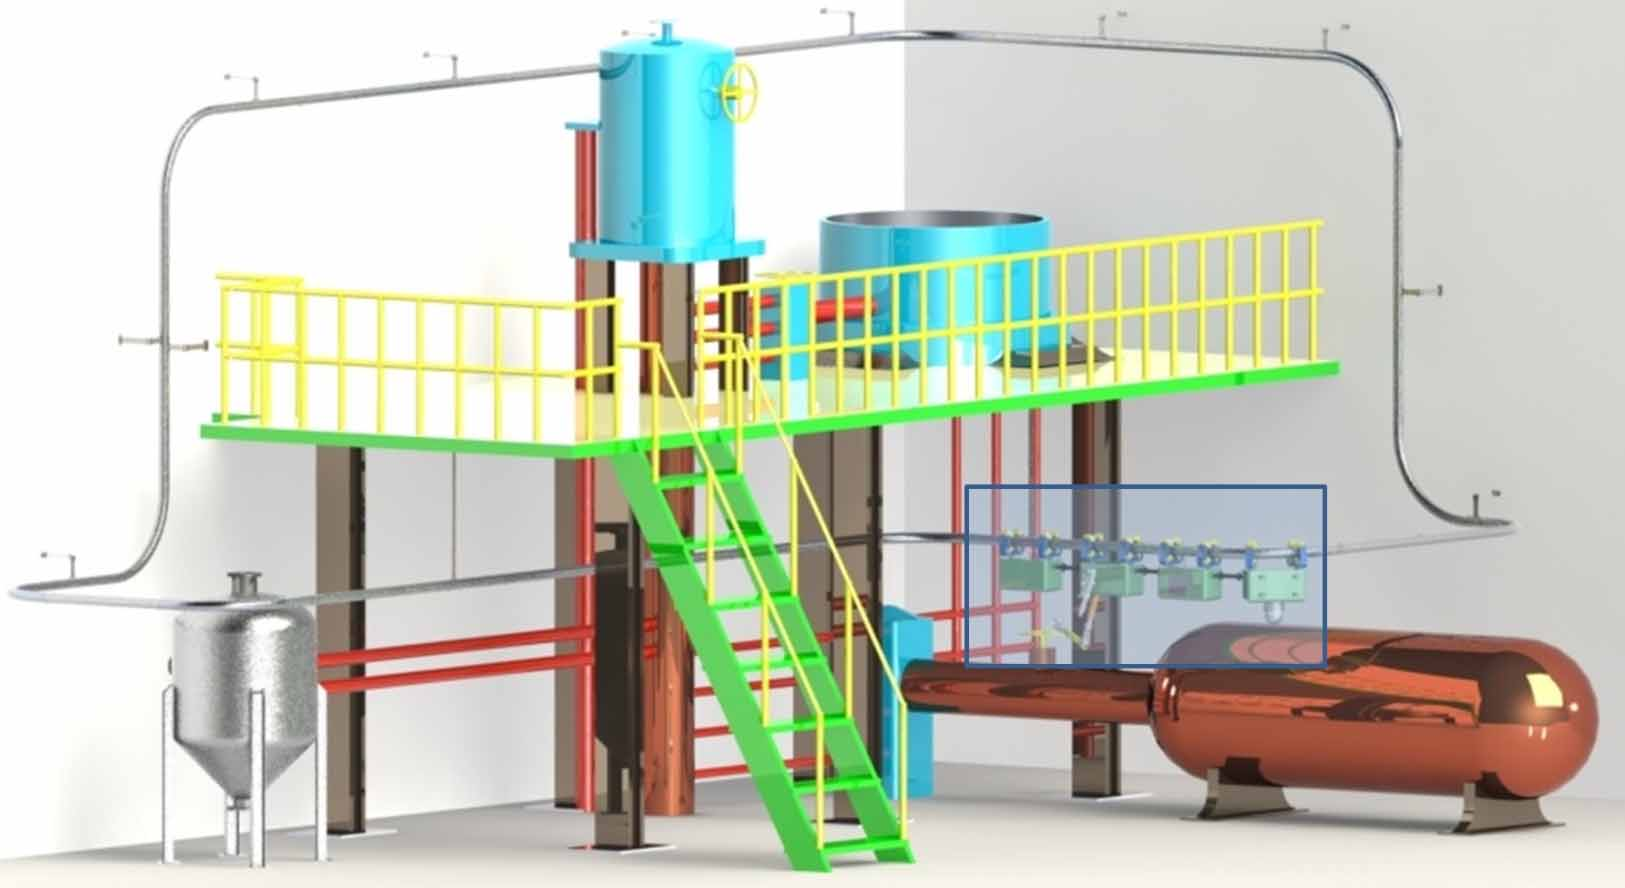
\includegraphics[width=8.4cm]{figs/cenario1.jpg}  % width is 7.6 cm.
    \label{fig:cenario1}}
\subfigure[Detailed zoom of the robot]{%
    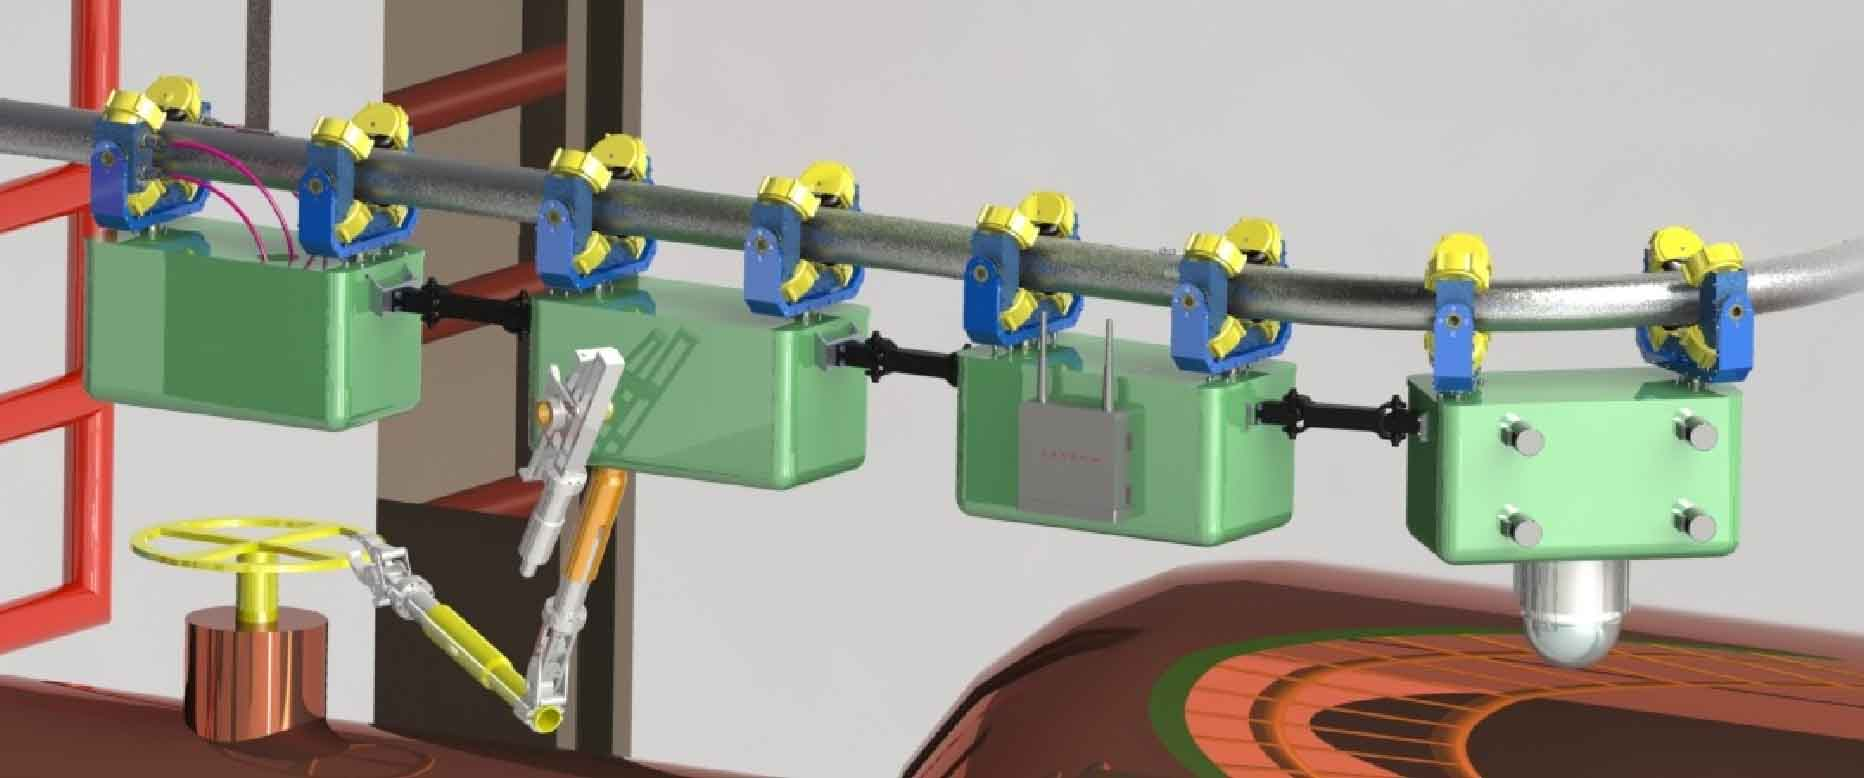
\includegraphics[width=8.4cm]{figs/zoom.jpg}  % width is 7.6 cm.
    \label{fig:zoom}}\vspace{-.1cm}
\caption{Illustration of the DORIS robot operating in a production plant.}\vspace{-0.25cm}
\label{fig:DORIS-overview}
\end{figure}

The DORIS project can be divided into five subsystems: electronics, power
supply, software, mechanics and signal processing.

%-------------------------------------------------------------------------------------------------------------------------
%ELECTRONICS
%-------------------------------------------------------------------------------------------------------------------------
% The electronics subsystem is responsible for providing embedded computational
% support for the robot control, signal processing, task managing, and local and
% remote communication. The device motion is controlled through drivers that can
% receive position, velocity, or current setpoints. The embedded electronics has
% two printed circuit boards for the vehicle support system: energy distribution
% and monitoring, basic failure detection, emergency handling and devices'
% control.

%-------------------------------------------------------------------------------------------------------------------------
%POWER SUPPLY
%-------------------------------------------------------------------------------------------------------------------------
% The power supply system uses military-class lithium-ion batteries, which have
% small size and high energy capacity. In the first prototype of DORIS, four
% batteries are used to power the motors and two to power the other electronics
% components.


%-------------------------------------------------------------------------------------------------------------------------
%SOFTWARE
%-------------------------------------------------------------------------------------------------------------------------
% The main objective of the software subsystem is to allow the implementation of
% high- and low-level control of the robot. The tools used to develop DORIS
% software architecture must consider two important factors: they have to be
% commercially available, and provide modular functionalities. These requirements
% led to the adoption of Qt as the graphical interface framework ~\cite{qt},
% Robot Operating System (ROS) as the communication middleware ~\cite{ros}, and
% Ubuntu as the operating system.
% 
% The software provides autonomous control (programmed tasks) and remote control
% through a Graphical User Interface (GUI) in the Host Control Base (HCB)
% computer. The HCB is composed of a set of processes running in parallel
% denominated ROS nodes, which can communicate with each other. To deal with this
% environment, a new software architecture called Robot Package Software is
% proposed, dividing the software into tools (graphical windows) and components
% (processing and communication unities), and grouping them into a dynamic
% library.

%-------------------------------------------------------------------------------------------------------------------------
%Mechanics
%-------------------------------------------------------------------------------------------------------------------------
The mechanical project designs the rail, the
traction and passive modules, and the joints used to couple them. The design
allows the robot to move smoothly in a 3D space and makes full stop anywhere
on the rail. Considering the severe corrosion and weather conditions in
offshore environments, the choice of materials are imperative to the success of
the project and certified solutions must be considered.

The robot is composed of two modules at its default configuration, but it is
conceived so that other modules can be added. The total weight of this
configuration is estimated at 50 kg and we expect to have a maximum speed of
1m/s.

The design incorporates the use of gimbals with wheels as guides for
the module on the rail. In the new configuration, the motors are
fixed on the gimbal and transmit its torque to the wheels via spur gears. The use of gimbals
is an proper choice concerning stability, guidance, and support. Furthermore,
it is possible to have a smooth vertical motion applying radial forces by the
clamping mechanism.

%-------------------------------------------------------------------------------------------------------------------------
%DSP
%-------------------------------------------------------------------------------------------------------------------------
The signal processing capabilities of the robot are: (a) Video: use
of multiple cameras (visible-light, infrared, fisheye and stereo) to detect
video anomalies such as abandoned objects, smoke, fire, liquid leakage, and
intruders. (b) Audio: detection of audio anomalies of impulsive nature, such as
an explosion or the diagnosis of rotating machines based on energy and pitch
(fundamental frequency) signatures using a single or a array of microphones. (c)
Vibration analysis: Use of acceleration sensors to diagnose the operation mode
of rotating machines, performing possible fault classification, such as
 misalignment and unbalancing operation. (d) Gas sensor: detection of gas
 leakages. (e) 3D mapping: environment 3D modeling using a laser sensor.

The main idea of all these signal processing features is to make the robot
perform an initial reference lap around the closed rail track, being manually
validated by a system operator. In the subsequent laps, all signal processing
algorithms compare the newly acquired signals with the reference data to detect
any form of anomaly, as indicated above. Once an anomalous behavior is
detected, an alarm is flagged to the system, which stores all associated data
for immediate or future diagnosis.


%-------------------------------------------------------------------------------------------------------------------------
%OTHER CHALLENGES
%-------------------------------------------------------------------------------------------------------------------------
Considering the robot functionalities and the aggressive offshore environment,
several challenges should be addressed. Temperatures in offshore facilities can
vary between $-30^{\circ}$C to $50^{\circ}$C, relative humidity can reach
100\%, and there may be splash water, salty air, storms, and high extensive
corrosion ~\cite{graf2007mobile}.

Concerning robustness and safety required to operate in classified areas, the
robot must be sealed against water and objects, resistant to a wide temperature
range, protected from impact and vibration, electrically shielded to avoid
explosion by ignition, and equipped with a monitoring system.


Another challenge is that the embedded computers must run heavy signal
processing algorithms, requiring high computational power. However, the power
supply subsystem must efficiently provide power and maintain a low level of
power consumption.

Further complications arise because the system is designed to move in confined
areas and have efficient wireless communication with operators, providing
online information of sensors data. Finally, the robot must have a modular and
flexible design, employing plug and play extensions.


\section{Embedded Electronics}\label{sec:electronics_overview}
The embedded electronics (EE) is composed of the following subsystems:
communication system, actuation system, vehicle support system, and
sensor integration system.

The \emph{communication system} is composed by: i) local Gigabit Ethernet network for massive data communication; ii) CAN (\emph{Controller Area Network}) for communication of control commands; iii) wireless technologies between the robot and the remote control base located at the offshore facility. DORIS can be remotely operated from this base via Wi-Fi IEEE 802.11n or via 2.4/5.0 GHz radio links (upon Wi-Fi failures).

The Ethernet network has a star topology centralized by a OSI-Layer 2 Switch, and connects DORIS main devices: i) computer; ii) three cameras (one with an embedded microphone); iii) Wi-Fi access point (another one is needed at the remote base); iv) \emph{Printed Circuit Boards} (PCBs). Together, Ethernet network and Wi-Fi form a \emph{Local Area Network} (LAN) for real-time communication and processing of massive data amount, such as audio, video, and images from all main cameras. In addition, this network topology allows the easy expansion of the Ethernet network for additional modules.

DORIS traction is taken by the \emph{actuation system}, which is composed by: i) 4 motor packs, each containing a EC brushless motor, an encoder and a
21:1 reduction gear; ii) 4 controller drivers; iii) respective cable/connector set. The actuation system is commanded by the DORIS computer via CAN bus, which provides reliability, transmission security and appropriate speed to this application. Since the traction system generates a significant amount of conductive noise, a galvanic opto-isolator is used between the CAN and the computer to minimize interference on the rest of the EE system.

Other peripheral devices may need USB communication, which is available at the
computer ports.

The \emph{Vehicle Support System (VSS)} is composed by microcontroller based
PCBs for: failure detection; device protection; energy distribution and
monitoring; emergency handling (\cite{MARIUS}). The VSS
functionalities is detailed further in subsection~\ref{sec:VSS}.

The sensor integration system is composed by all DORIS sensors and the interface
between devices and the computer. The subsystem enables inclusion,
reconfiguration and replacement of peripheral device. The sensor data
integration is carried out by an high performance Intel\textregistered
Core\texttrademark i7 computer embedded in a PCIe/104 form factor board.

An overall scheme of the EE system is shown at figure~\ref{fig:EE-Communications}.
\begin{figure}
\begin{center}
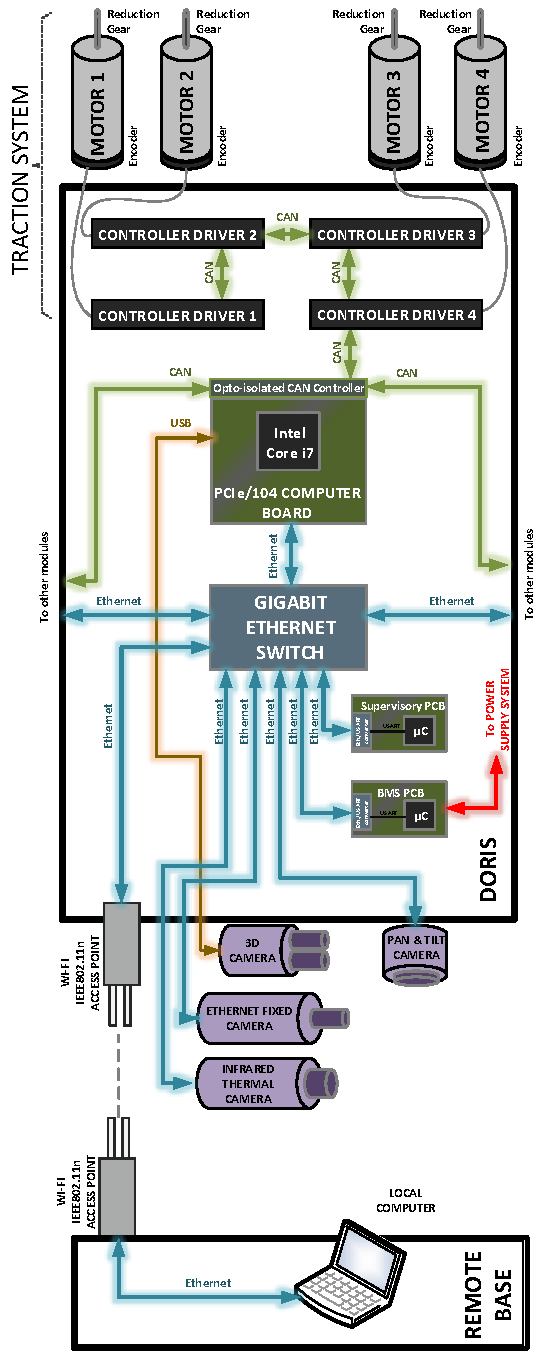
\includegraphics[width=8.4cm]{figs/EE-Communications.pdf}    % The printed column width is 8.4 cm.
\caption{Embedded Electronics system: overall scheme}
\label{fig:EE-Communications}
\end{center}
\end{figure}

\subsection{Vehicle Support System}\label{sec:VSS}

DORIS is equipped with a \emph{Vehicle Support System (VSS)} composed by microcontroller based \emph{printed circuit boards (PCBs)} for: failure detection; device protection; energy distribution and monitoring; emergency handling. The VSS functionalities are:

\begin{itemize}
    \item Failure detection is achieved by the monitoring of devices'
    current/voltage and module humidity/temperature.
    \item Peripheral devices are protected against overcurrent by fuses and
    solid-state relays, which can be turned on/off at any time automatically
    upon a detected failure or manually via operator.
    \item Energy distribution and monitoring is achieved by the \emph{Battery
    Management System (BMS)}. Each battery pack is monitored via SMBUS
    communication, which allows the reading of the battery status, voltage,
    current, temperature and remaining charge, besides other variables. This
    information allows the PCB embedded microcontrollers to provide adequate
    power balance in extreme situations (e.g.: demand of full power to either
    traction system or electronics system) or reconfiguration of power supply
    distribution in case of failures.
    \item In emergency cases, the robot can be turn on/off using a physical
    \emph{emergency shutdown (ESD)} button or via radio. The radio system can
    also replace Wi-Fi in some functionalities if it fails.
  \end{itemize}

DORIS VSS includes three board types: i) supervisory system
%(figure~\ref{fig:SSPCB})
; ii) Battery Management System - BMS
%(figure~\ref{fig:BMSPCB})
; iii) BMS Switching board%~\ref{fig:BMSSB}.

The supervisory system is mainly responsible for monitoring devices' current and voltage supply, and for protecting them. It is composed by AVR micrcontrollers, solid-state
relays (max. 1.5A), hall effect sensors (HES - for current measurements),
16-channels analog-to-digital converter (ADC), humidity/temperature (T/H)
sensor, and an Ethernet-to-UART converter.

The monitoring functions collects: i) module supply voltages, using the AVR embedded analog-to-digital converter; ii) module humidity and temperature, using an specific I$^{2}$C T/H sensor; iii) devices' supply currents, using hall-effect sensors and an external AD converter for data interpretation. Finally, the AVR manages the collected data in order to: i) periodically report it to DORIS computers (via Ethernet); ii) locally detect and react to faulty situations. Since Ethernet is not an available interface in this AVR model, an USART-to-Ethernet converter is used for data communication. The local fault detection is performed by pre-programmed algorithms in the AVR, which can react in order to protect devices against overcurrent. This is achieved by commanding the open/close of the relays, hence turning off the devices. All these AVR functionalities can also react to commands manually sent from the remote operator.

The BMS composition is similar to the supervisory system, with the following
differences: no solid-state relays for device on/off; no hall-effect sensors;
communication with batteries via \emph{SMBUS (System Management Bus)};
connection with the BMS bus switching board. The SMBUS is used to get important
information from the batteries, such as: temperature, voltages, currents and
remaining charge.

The BMS bus switching system contains high power solid-state relays (20A). They
can be commanded from the BMS AVR in order to adequate distribute the power to
either motor bus or electronics bus. The AVR decisions about the better
distribution is based primarily on data collected via SMBUS.

% \begin{figure}
% \begin{center}
% 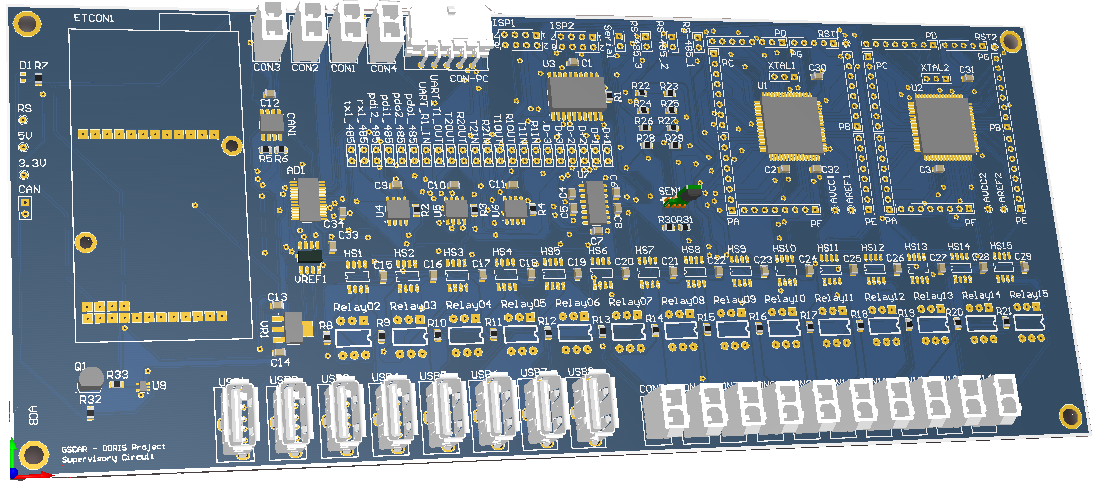
\includegraphics[width=8.4cm]{figs/SSPCB.png}    % The printed column width is 8.4 cm.
% \caption{Supervisory system PCB: 3D illustration}
% \label{fig:SSPCB}
% \end{center}
% \end{figure}
% \begin{figure}
% \begin{center}
% 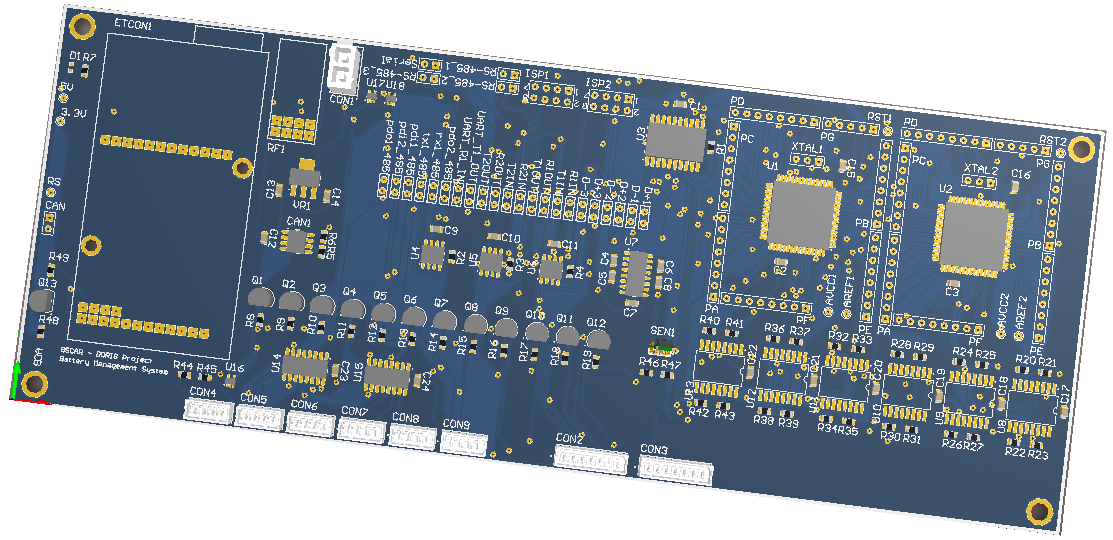
\includegraphics[width=8.4cm]{figs/BMSPCB.png}    % The printed column width is 8.4 cm.
% \caption{Battery Management System PCB: 3D illustration}
% \label{fig:BMSPCB}
% \end{center}
% \end{figure}
% \begin{figure}
% \begin{center}
% 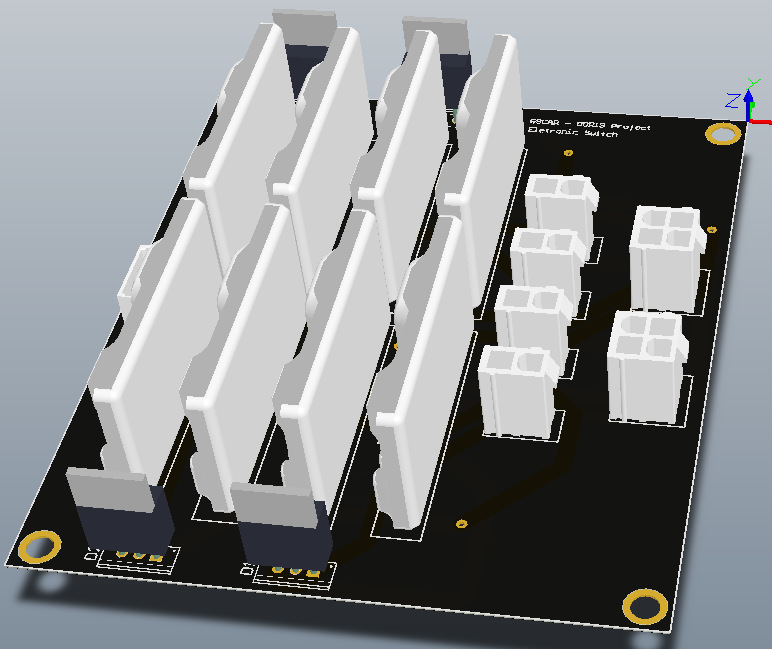
\includegraphics[width=8.4cm]{figs/Top2.png}    % The printed column width is 8.4 cm.
% \caption{Illustration of the Power Bus Switching Boards Options.}
% \label{fig:BMSSB}
% \end{center}
% \end{figure}
\section{Power supply system}\label{sec:powersupply_overview}
This system is responsible for the safe, reliable, and efficient electric power distribution for DORIS parts. The power is supplied by high
density energy level military lithium ion battery technology, which comes with
an intrinsically safety circuit for protection against short-circuits and heating. Each battery pack support has a capacity of 10 Ah. According to mechanical constraints, each DORIS module admits a maximum of four battery packs, each one weighing 1.4 kg.

As Verma \emph{et al.} (2004) highlights, robots often operate in environments
where human intervention is expensive, slow, unreliable, or impossible. Therefore, it is essential to monitor their behavior so that faults may be addressed before they result in dangerous failures. For proper power management, the electronics system uses information about each battery condition, such as battery voltage, current, temperature and remaining charge. This data is read by the PCB microcontroller from the batteries via System Management Bus (SMBUS) protocol, as described further in section \ref{sec:VSS}.

In order to avoid electromagnetic (EMI) and conductive noise interference, the project
currently works with two separate power buses, each of these built using two
24Vdc batteries connected in parallel, being able to deliver a capacity of
20Ah. One bus is dedicated to power the motors and the other to power all
electronic devices. Also, DC/DC converters are
being used to create different voltage levels (12Vdc and 5Vdc) and to
ensure a stable power source (even for 24Vdc components).

Seeking power protection, Diodes are being used in order to avoid back-flow
current, fuses are protecting the system from undesired peaks just after each
DC/DC converter and buttons allow power buses to be separately turned on/off.


The current architecture of the power supply embedded on this project is
illustrated on figure~\ref{fig:DiagramaSAM}. The electronics' power bus uses
14AWG wires for up to 15A of nominal current and the motors' uses
12AWG wires for up to 21A of nominal current.

Since the source from this system is a DC battery, there is no need for a
capacitor in order to correct a delay between current and voltage as there will
be no natural frequency. However, a capacitor bank would allow additional
energy to motors, providing sufficient current. If the source energy is a
battery then the capacitor bank must have at least 400 to 500 $\mu F$ for each
Ampere. In our case, as each motor may require a peak current of 20A, a
capacitor bank dedicated for each driver would need to have between 8000 and
10000 $\mu F$, where smaller capacitors should be used in parallel. It is also
recommended to have the maximum operating voltage of the capacitor bank at
around 50\%, ie, 35V (trade) since the battery voltage is 24V. In this case,
one must use electrolytic capacitors, since other types of capacitors are not
able to provide this capacitance value at this voltage.
The capacitor should have low ESR (equivalent series resistance - Equivalent
series resistance). Furthermore, it should be located as close to the noise
source, namely the motors.

\begin{figure}[ht]
\centering
%\subfigure[Robot's operational scenario in a production plant]{%
    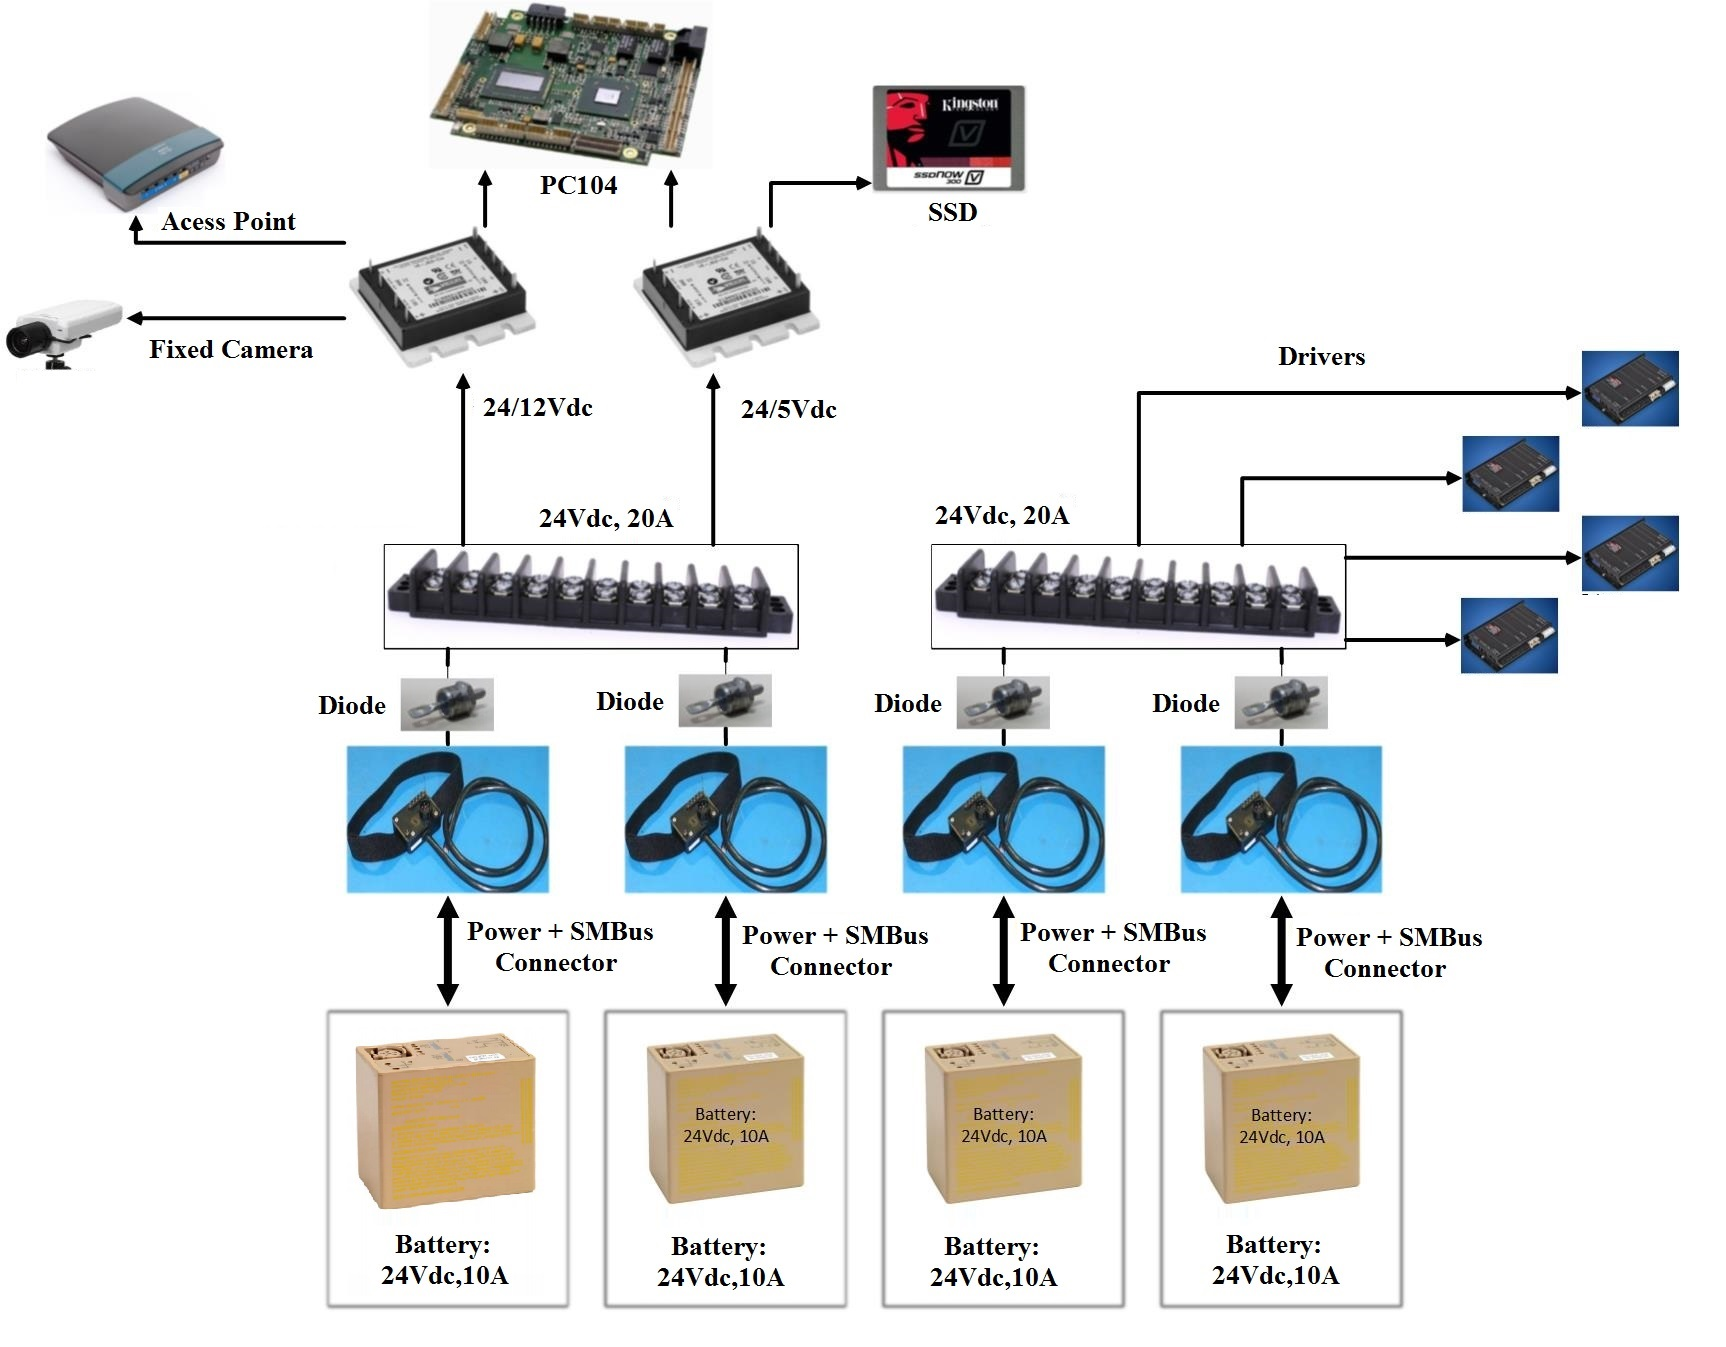
\includegraphics[angle=90,width=1\columnwidth]{figs/DiagramaSAM.jpg}  % width is 7.6 cm.
    \label{fig:DiagramaSAM}
\caption{Power Supply Architecture.}\vspace{-0.25cm}
%\label{fig:DORIS-overview}
\end{figure}

Considering this, new challenges came up in order to improve the features of
the system.
\section{Experimental tests and results}\label{sec:results}
A DORIS prototype called \emph{Single Autonomous Module} (SAM) was built for tests of all concepts above. In addition, some VSS functionalities were individually tested, but not yet fully integrated with SAM. The two subsections below detail the tests.

\subsection{Single Autonomous Module (SAM)}
SAM (figure~\ref{fig:SAM2}) is composed mainly by an ethernet fixed camera, USB 3D webcam, wireless router, motor and drivers, a PCIe/104 computer module with \emph{solid-state drive} (SSD) and few PCBs. It was tested in horizontal and vertical motion on a rail composed of straight and curved modules. A tubular track built using straight and curved segments was installed in the GSCAR laboratory, in COPPE/UFRJ. The track comprises all possible movements that the robot must make.

The first objectives of SAM is to test the following concepts:
\begin{itemize}
  \item Power supply: independent buses for motors and electronics devices;
  batteries robustness and duration;
  \item Electronics: sensor integration; communication system;
  \item Software: teleoperation; user interface.
  \end{itemize}

% \begin{figure}[!h]
% \begin{center}
% 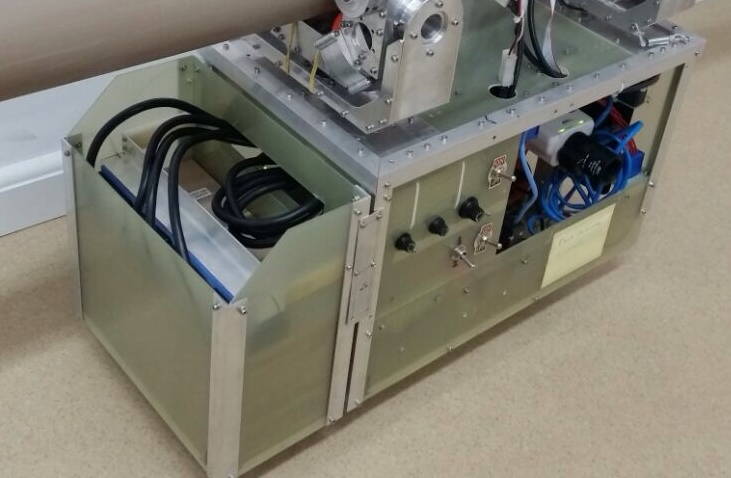
\includegraphics[width=8.4cm]{figs/SAM1.jpg}  % width is 7.6 cm.
% \label{fig:SAM}
% \caption{Single Autonomous Module}
% \end{center}
% \end{figure}
\begin{figure}[!h]
\begin{center}
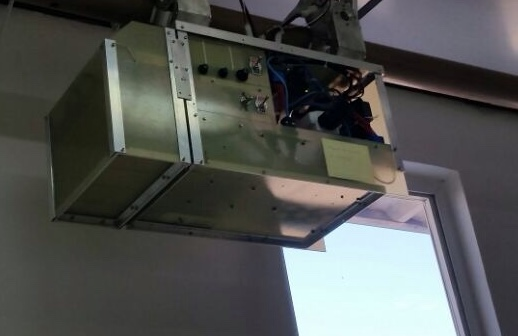
\includegraphics[width=8.4cm]{figs/SAM2.jpg}  % width is 7.6 cm.
\label{fig:SAM2}
\caption{Single Autonomous Module}
\end{center}
\end{figure}

%-------------------------------------------------------------------------------------------------------------------------
%TESTES/RESULTADOS
%-------------------------------------------------------------------------------------------------------------------------
%Initial tests performed with the prototype show good performance of the gimbals
%in terms of stability. Even though the gimbals may shake slightly due to
%irregularities on the rail surface and asymmetrical positioning of the guide
%wheels, the base keeps a steady orientation while moving.
The concept of independent power buses proved to be efficient, and the designed battery capacity could handle the system energy demand. It was observed that when SAM moves downwards, the motor generates energy. Depending on
the fall height and the SAM velocity, this energy may reach a voltage level that causes the motor drivers reset.

The implemented communication networks were: i) Ethernet, to connect the fixed camera, the PCIe/104 and the access point; ii) Wi-Fi, to connect SAM with the base; iii) CAN, to control the actuation system; iv) USB, to connect the 3D Webcam. The communications worked properly as expected.

SAM is current located at GSCAR lab, in Federal University of Rio de Janeiro, Brazil. It can be teleoperated from anywhere by accessing its Wi-Fi network and the GUI (\emph{Graphical User Interface}) developed in Qt environment. SAM has already been teleoperated from CENPES/Petrobras (Rio de Janeiro) and from Statoil headquarters (Norway).

\subsection{Vehicle Support System Tests}
<<<<<<< HEAD
All DORIS VSS functions were successfully tested independently. For these
tests, it was used a test PCB (similar to the designed for the final prototype)
and a RS485 interface with a laptop to emulate the USART communication. The AVR
microcontroller, which commands all the PCB functionalities, were programmed in
C++ using Atmel Studio 6.1. The following tests/implementations were
successfully performed:

\begin{enumerate}[i)]

\item Logic for commanding the \emph{solid-state relays} for device on/off: the
relays can be opened/closed via RS485 commands from the laptop.

\item Acquisition of \emph{module voltages}: DC-DC voltage measurements (5, 12
and 24VDC) and battery raw voltage measurement (that does not pass through any
DC-DC) can be read via RS485 commands from the laptop. The voltage is measured
using the AVR embedded AD converter.

\item Acquisition of \emph{module currents}: the measurement of currents that
supply each device module can be read via RS485 commands from the laptop. The
currents are measured using hall-effect sensors. The microcontroller embedded
AD converter does not comport enough measuring port, thus an external one is
used to digitize the current measurements.

\item Acquisition of \emph{module humidity/temperature}: the measurements of
the module humidity and temperature can be read via RS485 commands from the
laptop. A specific T/H sensor is used for this acquisition.

\item Acquisition of \emph{battery information}: many battery information, such
as voltages, temperature, currents, remaining charge, and battery status, can
be read via RS485 commands from the laptop. The acquisition of all battery data
is implemented using SMBUS communication.

\end{enumerate}



=======
All DORIS VSS functions were successfully tested independently. For these tests, there were used a test PCB (similar to the designed for the final prototype) and a RS485 interface with a laptop to emulate the USART communication. The AVR firmware was programmed in C++ using Atmel Studio 6.1. The following tests/implementations were successfully performed:
\begin{enumerate}[i)]
\item Logic for commanding the \emph{solid-state relays} for device on/off: the relays can be opened/closed via RS485 commands from the laptop.
\item Acquisition of \emph{module voltages}: DC-DC voltage measurements (5, 12 and 24VDC) and battery raw voltage measurement (that does not pass through any DC-DC) can be accessed via RS485 commands from the laptop. The voltage is measured using the AVR embedded AD converter.
\item Acquisition of \emph{module currents}: the measurement of currents that supply each device module can be read via RS485 commands from the laptop. The currents are measured using hall-effect sensors. The microcontroller embedded AD converter does not comport enough measuring port, thus an external one is used to digitize the current measurements.
 \item Acquisition of \emph{module humidity/temperature}: the measurements of the module humidity and temperature can be read via RS485 commands from the laptop. A specific T/H sensor is used for this acquisition.
\item Acquisition of \emph{battery information}: many battery information, such as voltages, temperature, currents, remaining charge, and battery status, can be read via RS485 commands from the laptop. The acquisition of all battery data is implemented using SMBUS communication.
\end{enumerate}
Future challenges include: replace RS485 by USART to allow communication with the PCs via Ethernet network; implement in AVR the control of BMS high-power relays to permit the management of DORIS energy power distribution; implement the logic that uses the data read from SMBUS to manage DORIS energy distribution. Additionally, timers will be implemented to permit: robot shutdown in predetermined time; sending of periodic data report of voltages, currents, relays’ status, and module humidity and temperature.

%Finally, the traction system mounted on a prismatic mechanism did not work properly. The prismatic joints locked in certain circumstances and the weight of the traction system led to loss of contact between the lower part of the grooved wheels and the tube. This results suggest investigating an alternative concept for the traction system, for example moving the traction to the gimbals wheels, as presented in Section \ref{sec:mechanics_overview}.
>>>>>>> refs/remotes/origin/master
\section{Conclusion and Future work}\label{sec:conclusions}

In this paper, we presented the DORIS project, which endeavors to develop an
offshore facilities inspection and monitoring robot. The prototype is based on
rail guided modules powered by a battery system and equipped with multiple
sensors that enable detection of anomalies, such as abandoned objects and gas
leakage.

A prototype, SAM, was built to test electronics, power
supply, and software architecture concepts.
Preliminary results show good overall performance of: i) sensor integration and communication; ii) independent power buses for
electronics and motors; iii) teleoperation.

%Thus, DORIS is equipped with a power supply system with an improved robustness
%level when compared with other robotic systems and it also has a considerable
%light weight, high energy density and increased safety properties.

The Vehicle Support System was tested outside the robot and the customized
printed circuit boards were able to monitor: the batteries via SMBUS,
temperature/humidity, DC/DC voltage levels, and devices's currents. The
solid-state relays can also turn on/off the devices for protection and/or
efficiently power consumption.

Ongoing implementations and future challenges include:
\begin{enumerate}[i)]
  \item \emph{Expansion and reconfiguration of robot modules}:\\
  \newline
  DORIS will need more than one module to support more devices and features.
  The EE system permits the free expansion and reconfiguration of DORIS
  modules, achieved by the introduction of a bus topology for DORIS
  main networks: Ethernet and CAN.\\
  \item \emph{Autonomous operation}:\\
  \newline
  DORIS autonomous operation is a challenge for the software development. The
  Positioning System, comprising wheels' encoder (odometry) and
  fixed camera (3D mapping), will be upgraded with an inertial movement unit
  (IMU) and a laser scanner. The sensor's fusion will precise the Navigation
  System, which estimates the linear position and velocity of the vehicle. Also,
  a Mission Control System need to be developed for the operator.\\
%  \item \emph{Manipulator control}:\\
%  \newline
%  It is planned the inclusion of a robotic manipulator fixed at the module
%  bottom. It is going to handle a vibration sensor and a 3D camera at the grip.
%  Besides the prismatic movement of the robot along the rail, the manipulator
%  may need more 4 degrees of freedom, excluding the \emph{roll orientation}.
%  Since it is actuated by electric motors just like the traction system, it
%  will be controlled via CAN bus.\\
  \newline
  \item \emph{Reduced interferences, such as Electromagnetic interference (EMI) and electrostatic charge}:\\
  \newline
  Future DORIS improvements should include a well designed/installation of the
  shield network and grounding system to reduce EMI. An electrostatic discharger
  should be designed to drain the accumulated charge from the shielding system.\\
  \newline
  \item \emph{Solution for DORIS's downward motion issue}
  \newline
<<<<<<< HEAD
  The digital processing is working on an audio filter for the DORIS motors,
  which generates a lot of noise when working at higher speeds.
  \item \emph{Vehicle Support System}
  \newline
  Functions to be implemented in VSS: control of BMS high-power
  relays to permit the management of DORIS energy power distribution;
  The logic that uses the data from SMBUS to efficiently manage DORIS's energy
  distribution; Robot shutdown in predetermined time; Periodic data
  report of voltages, currents, relays� status, and module's humidity and
  temperature.
=======
  The regeneration issue impose an overvoltage on the drivers, that resets for a
  while during the robot movement downwards. To prevent it, a shunt regulator
  may be used in order to dispose of the extra energy and avoid the over
  voltage issue. It represents a solution, but wastes this energy, where in
  this case a bigger capacitor bank could also work as an energy storage
  device. Tests are going to be performed so that the amount of energy
  generated may be measured in order to decide if it would be worth to embark a
  device to recover this energy or if it would be better just to let it be
  wasted.
  \item \emph{Hardware Certification}
  \newline
  The robot must be explosive-proof, weather-proof and salt-water-proof, and the
  electronics must be suitable for harsh environments.
>>>>>>> refs/remotes/origin/master
\end{enumerate}

\bibliography{ifacconf}

\appendix

\end{document}
